\documentclass[12pt]{report}
\usepackage[utf8]{inputenc}
\usepackage{graphicx}
\usepackage{amsmath}

\title{Electronic Warfare, principles and fundamentals}
\author{Ivan Riolo}
\date{November 2020}

\begin{document}
\maketitle
\tableofcontents


\chapter{Introduction} 
Electronic warfare is defined as the set of all the practices and actions undertaken by means of weapon systems, in order to attack enemy electronic systems, defend and support them.
All these practices are possible by exploiting the technology of modern warfare systems, considering the on-board presence of electronic equipment and their radio/electro optic/infrared operation which obviously involves the use of the electromagnetic spectrum (EM spectrum). In fact, the main concept that give us a clear explanation of electronic warfare is based precisely on it, the ability to guarantee access and correct exploitation of the electromagnetic spectrum to friendly systems at the expense of enemy ones. In the EM spectrum is possible to sense and analyze adversary's applications to understand which actions enemy does and how he does its, then is possible to apply an appropriate countermeasure specific for that enemy's action. Therefore EM spectrum is the battle ground in EW and all its practices are possible thanks to use of sensors, radars and sophisticated systems (most of them already present in this scenario for classic war action) that made possible to sense, analyze and produce a response. Defined the operational environment, the applications of EW took place in two main category, points defense weapon systems in which the instruments are set to defense a small geographical area approximate by a point and territorial defense weapon systems where the region to defend is a non negligible volume value. These are subdivided into four main different contexts: air, sea, land and space, where EM spectrum is exploited for command and control, weapon targeting and weapon control. With these EW practices that can involves all the instruments that use the EM spectrum, is mainly possible to contrast enemy's action and also to target humans, telecommunications, radars and more in general all the electronic instruments. 


\section{EW subdivisions}
The EW actions are divided into three principal components, each component contains all the specific technique and instruments used for that category, these are:
\begin{itemize}
\item Electronic Attack (EA), also called Electronic Counter Measure (ECM);
    \begin{itemize}
      \item Is worth noting that in the EW vision the attack is considered a countermeasure to an enemy action, while by the external point of view it is a defense action. 
      \end{itemize}
\item Electronic Protection (EP), also called Electronic Counter Counter Measure (ECCM);
    \begin{itemize}
      \item which protect own electronic systems and their signal transmissions above EM spectrum against intercepting and signal intelligence of enemy.
      \end{itemize}
\item Electronic Support (ES), also called Electronic Support Measure (ESM);
    \begin{itemize}
     \item which provides warning and surveillance information by intercepting enemy's signals from EM environment.
     \end{itemize}
\end{itemize}
These three components usually are correlated and used/implemented together, in real or delayed time, in order to understand what and how enemy does (electronic support/signal intelligence), then to produce countermeasure action to contrast it (electronic attack) and at the same time to protect own electronic systems against enemy's signal intelligence (electronic protection). The actions made by weapon systems are also subdivided in three category or phase listed below:
\begin{itemize}
     \item Research and acquisition:
     \begin{itemize}
        \item The preliminary phase to EA (Electronic Attack), the ES (Electronic Support), in which many surveillance system (SIGINT) analyze the space looking for a possible threat (also multi threat detection), then identify and evaluate it so will be possible to decide which Electronic Counter Measure should be produced. Are used optical sensor, and other instruments called Electronic Support Measurements.
        \end{itemize}
    \item Contrast:
        \begin{itemize}
            \item The phase in which the EA (Electronic Attack) are physical produced after decision taken in precedent phase. Are used many possible different sensors to engage the threat and then typical weapons to produce the offensive response, but most important by the point of view of EW are the directed energy weapons or the means of disturbance and deception.   
        \end{itemize}
    \item Weapon system's management:
        \begin{itemize}
            \item The phase in which the actions of ES (Electronic Support) took place for manage and control all the operations and also for communications or data exchange between the several systems.
        \end{itemize}   
    \end{itemize}
   
In each phase it's possible to distinguish the different instruments/systems that are used. For example in the acquisition phase are used electromagnetic and optical sensor (infrared, laser and radar) like coherent doppler pulse radar or Identification Friend or Foe system (IFF) . In the contrast phase are used coherent doppler pulse tracking radar to engage the target, typical offensive means and disturbance or deception means to disable the enemy's offensive. While in the management phase are used telecommunications systems and more in general Human Machine Interface (HMI) or Man Machine Interface (MMI) that simplify the interaction between the user and the system. Another important systems classification of electronic warfare is proposed in the following scheme \ref{EWsubdivision}. It's possible to divide all the systems in two main category: real time and delayed time. 
Usually in real time category there are the emergency systems that requires an instant application. Belongs to this category all the subdivision precedent explained (EA, EP, ES) while operation like the signal intelligence can be applied also in a delayed time. The principle aim of this category is to take information or data about 'intercepted signals' to 'know' what instrument/device is used by the enemy and better decide which countermeasure is possible to adopt. It's possible to refer at signal intelligence (SIGINT) in a specific way for the weapon system with the name electromagnetic intelligence (ELINT), the prerogative in this case is to analyze and exploit the electromagnetic spectrum. It's possible to refer in a specific way also to the communications with the name communication intelligence (COMINT), in this case the prerogative is to intercept the communications message of enemy. 

\begin{figure}[h!]
    \centering
    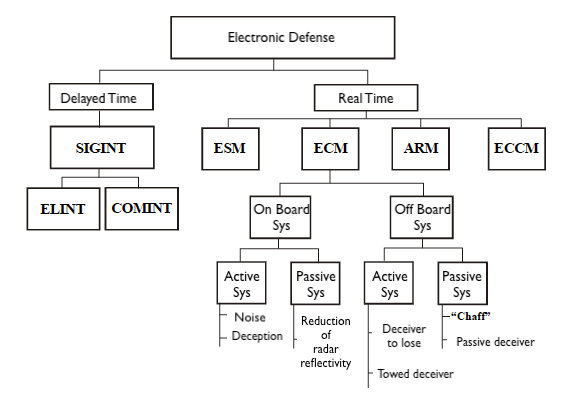
\includegraphics[width=12cm]{Pictures/EW subdivision.png}
    \caption{EW subdivision}
    \label{EWsubdivision}
\end{figure} 

The ESM (Electronic Support Measurements) category is the first group of real time system and it is composed by all the devices used to alert with early warning possible threats by scanning continuously the EM spectrum.
Typical device for this purpose is the Radar Warning Receiver (RWR), that send an alert when detect a possible enemy radar signal in the spectrum (for example an enemy guided weapon that use a tracking radar to follow the victim). \newline The ECM (Electronic Counter Measures) or EA (Electronic Attack) is the category in which there are all the systems that use electromagnetic energy in turn to limit or deny enemy threat (ex. disruptive action against enemy radar). In general the ECM systems are divided in two groups, 'on-board' ECM in which the system have an active part (ex transmitter to disrupt radar enemy signal, belongs to this category noise jammer and deception jammer like self screening jammer, stand off jammer and escort jammer, see cap. \ref{Electronic Attack}). There is also a passive component like 'signature reduction' in the case of 'on-board' system (stealth technology to reduce radar cross section by select specific geometry and materials). Then there are the 'off-board' ECM category in which more than an active stand-alone system (active means that transmit energy) can be also a passive component that in this case can be 'decoy' (electromagnetic reflective object, corner reflector) or 'chaff' (cloud of metallic object reflective). \newline Another category of real time systems is the ARM (Anti Radiation Missile) category in which are classified all the systems used for physical contrast of enemy electromagnetic source with self-guided missiles. Is important to note that in this case the electromagnetic component play a key role because also if the contrast is physical by means of missile, that weapon is guided by receiver tuned on the electromagnetic emitter. Finally the Electronic Counter Counter Measure (ECCM) is the category in which there are all the system used to contrast ESM and ECM capacity of enemy, simply by using the equivalent symmetric ECM system that must be contrasted. In the figure below is shown typical point of an aircraft where are installed the radar warning receiver, and the typical user interface of such device.
\begin{figure}[h!]
    \centering
    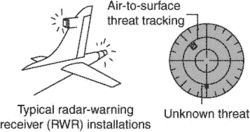
\includegraphics[width=8cm]{Pictures/RWR.jpg}
    \caption{EW subdivision}
    \label{EWsubdivision}
\end{figure} 
\newpage    
\section{Electromagnetic enviroment}
The electromagnetic spectrum are defined like a battlefield, so the scenario of all the arguments in EW, in fact all the actions starts from ES context (surveillance, identification), EA and EP involve the use of it by employing signals transmission and reception devices. It is worth nothing that in normal communications scenario all the features of used signals are known a priori so it's very simple to design devices of transmission and reception that are extremely efficient. In EW context all the signals that ES's systems wants to detect and reveal are unknown a priori so is impossible to achieve extremely efficient devices. The most disabling issue is the bandwidth of signals that systems are looking for, if it is not known, the surveillance devices must be tuned with a very big set of frequencies. So the 'instant band' (the set of frequencies with which the receiver works simultaneously) must be wide as coverage band (the set of all possible frequencies with which the receiver can work), in this way all the signals of no interest reach the device and became difficult to discriminate signals of interest. The radar environment belongs to EM spectrum and it's composed by all possible signals that a radar device of a system weapon can transmit. The systems that research information across the EM spectrum belong to SIGINT (SIGnal INTelligence) branch. To better understand a radar's carrier is RF (Radio Frequency) signal and it is CW (Continuous Wave) signal in case of pulse amplitude modulation otherwise is a pulse signal. Is important to consider that CW signals can operate with low energy level and in this case are difficult to detect, consequently is increased the Low Probability of Intercept (LPI) parameter. The principle device that is used to exploit EM spectrum and to understand what is going on, obviously is a receiver device. It's main parameter, the opposite of last one seen (LPI), is the Probability of Intercept (POI) parameter. POI is the probability that given a presence of a signal on the EM spectrum it is correctly detected. This parameter is related to the 'instant band' in turn related to the thermal noise, and the sensibility in turn related to the minimum SNR (Signal to Noise Ratio). Consequently the parameters 'instant-band' and 'sensibility' are in contrast because increasing of the instant-band means reducing of the SNR and so the sensibility. For this reason there are two group of receiver, respectively named "wide open" and "super het" receiver. In the first one category the instant-band is equal to the coverage band and for this reason the sensibility is not too high. In the second category, "super het", the instant band is only a fraction of the coverage band e so the sensibility can be high. But this trade off between instant band and sensibility is balanced by the fact that with the full band devices (wide open) the POI parameter is max (POI = 1) while with only a fraction of full band (super het) the POI parameter is low (POI \textless 1, the target which receiver are looking for is in a portion of EM spectrum that it's not tuned). How it is possible to understand the branch of ES plays a key role in the EM spectrum environment. The big problem that limits the performance of used devices is the high density of signals simultaneously present in the EM spectrum, such one million of pulses per second in all bandwidth of interest so there is an high probability of overlap. The solution to this problem is given by a subdivision of bandwidth in reception with parallers receivers. (See later \ref{Systems})
\begin{figure}[b!]
    \centering
    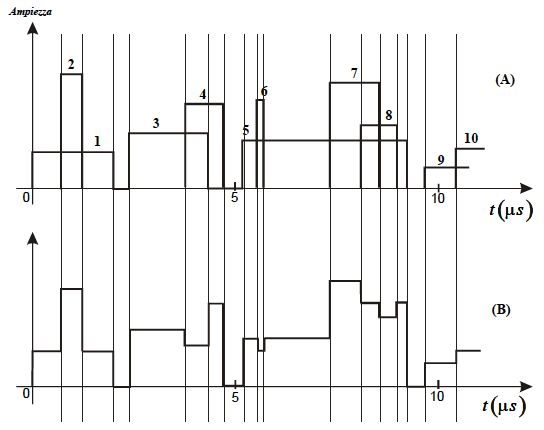
\includegraphics[width=12cm]{Pictures/BW subivision.png}
    \caption{Superimposed signals}
\end{figure}

\newpage
\section{Motivation and goals}
The first documented use of EW approach goes back to the Russo Japanese war in 1904, when the Japanes auxiliary cruiser localized with radar approach the Russian fleet. The first admiral of Russian fleet tried to disturb the wireless communications of Japanese auxiliary cruiser by using a jamm approach without success and led Russian to defeat. Already one half century ago, during the second World War, the sophistication of EW systems and in particular of threat systems is shown with use of infra-red guided surface to air missiles and radar guided anti aircraft. Winston Churchill referred to as the "Battle of the Beams". This first used devices based their technology on superheterodyne receivers, klystron and magnetron sources of signals and vacuum tube amplifiers. In the beginning the radio transmission (RF) of confidential information like troop disposition and so on was intercepted to prevent the enemy's operations. Also if the messages were encrypted at least was possible to localize the source of transmission with triangulation technique. Then another important conceptual introduction of EA was proposed by using radar systems and other devices to inject microwave energy into the EM spectrum environment, so not only was possible to understand what enemy was doing and where, but also to modify their perception of surroundings. With improved technology of communications and radar systems EW played a major role in main military operations like in Vietnam War. The evolution of devices signed by the passage from super het and crystal video receivers to to wideband channelized receivers coupled with precision receivers led to a rapid analysis of EM environment and at the same time with a very good accuracy. An example of this modern electronic warfare approach is proposed in 2010 bu Russia with multifunctional electronic warfare system known as Borisoglebsk 2. It is composed by four different jamming stations and with this instruments achieve the successful suppression of mobile satellite communications and satellite navigation signals. 

\newpage
\chapter{Systems, sensors and antennas} \label{Systems}
In this section are described the main categories of receivers, the starting devices of all EW actions. Then is explained the technological evolution of that category with describing the best solution of system with an implementation of antenna's array to incorporate all the EW actions in one single system. 
\section{Crystal video receiver} The simplest possible implantation of a receiver is offered by the Crystal video receiver, is a Wide-Open solution (Instant band and coverage band are coincident). It is composed by four component below described and is important to nothing that with this implementation is not possible to measure signal's parameters but it is used only as detector:
\begin{itemize}
     \item Antenna: 
         \begin{itemize}
         \item Usually an omnidirectional antenna to perform a detection among all the coverage bandwidth.
         \end{itemize}
    \item Crystal detector: 
         \begin{itemize}
         \item composed by a diode.
        \end{itemize}
    \item Video amplifier:
         \begin{itemize}
         \item To amplify the signal in the whole bandwidth.
         \end{itemize}
    \item Comparator:    
         \begin{itemize}
         \item To compare the signal detected with a threshold, if it is above the detection is confirmed, otherwise the detection abort.
         \end{itemize}
\end{itemize}

Is important to note that with this configuration is possible to achieve unitary value for the POI parameter. On the other hand is possible to increase also the sensibility, that is low because of the use of whole bandwidth (wide open), by inserting a pre amplifier RF. This solution in not preferred because is very complex to implement an amplifier for a very large band RF which keeps its parameter constant. A variant of Crystal video receiver is proposed by the tuned crystal video, that is no longer a wide open device, but it is a frequency tunable device. This configuration is possible by inserting before the detector a RF filter that select the portion of interested bandwidth. The result is an increment of the sensibility against the POI parameter that is minor than one (instant bandwidth is no longer the whole coverage band, but a fraction of it). A scheme with typical parameters value of this receiver is shown in the next picture.

\begin{figure}[h!]
    \centering
    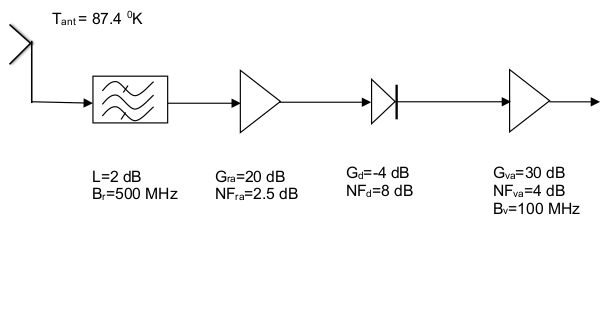
\includegraphics[width=12cm]{Pictures/Crystal video receiver.png}
    \caption{Crystal video receiver}
\end{figure}

The worst cons of  crystal video device are:
\begin{itemize}
         \item Impossibility to detect CW signals and to perform measurements to detected signals;
         \item Impossibility to manage simultaneous signals, because it's impossible to discriminate its in frequency.
\end{itemize}
 
\section{Super het receiver}  
A solution to previous described problems is proposed by the Super het receivers. This receivers are the most used devices in EW. In particular this type of receivers solves the problem of pre amplification, that in the whole RF band is difficult, by translate the received signal in an intermediate frequencies (IF) band. This last one is only a fraction of the whole bandwidth and makes simple to perform any kind of operation such amplification. So the new implementation provides a first stage after antenna, composed by a mixer and a local oscillator that performs the translation of the received signals. Then the filtering operation is performed in IF to select the target band and follow the IF amplifier. In this way the only influential source of noise is the mixer, to prevent it is usual inserted a pre amplifier RF before the IF conversion. So the components of super het reciver are in order the following:
\begin{itemize}
         \item Antenna;
         \item RF amplifier;
         \item RF filter;
         \begin{itemize}
            \item To prevent the possible intermodulation phenomenon, when an high power signal arrives to the pre amplifier and 'saturates' it.  In this case the intermodulation allows the possibility to introduce non interesting frequencies in the IF conversion (mixer). Filter is solution to prevent this phenomenon by select only the correct set of frequencies.
         \end{itemize}
         \item Mixer plus Local Oscillator;
         \item IF filter;
         \item IF amplifier;
         \item Diode detector;
\end{itemize}
\begin{figure}[h!]
    \centering
    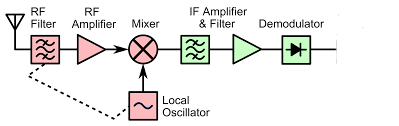
\includegraphics[width=12cm]{Pictures/super het receiver.png}
    \caption{Super het receiver}
\end{figure}

Pros of this implementation are, first of all, the possibility to amplify the signal of interest in a restricted band to achieve a good sensibility. Then the possibility to make different measurements to it, in such a way that is possible to manage simultaneous signals thanks to discrimination, for example in frequencies. For this purpose is shown now the IFM (Instantaneous Frequency Measurements) receiver.
\section{IFM receiver} It's principal goal is to measure the instantaneous frequency of received signal. The key concept of this device is given by a delay line put in parallel to an undelay line after the receiver antenna, so that knowing the delay parameter is possible to measure the phase difference between the two signals (the one delayed and not). Note that the phase is: $\Delta \phi = 2 \pi f_{0} \tau$ and became very simple at this point to obtain the frequency value. This is possible by passing the two signals to a phase correlator which practically makes the product between $exp(-2 \pi f_{0} t)$ and $exp(2 \pi f_{0} (t + \tau))$. The four exits of correlator are then passed to a couple of differential amplifier in such a way that the two result at the output are: 

\begin{itemize}
         \item E = 2 $\sin{2\pi f_{0}\tau}$
         \item F = 2 $\cos{2\pi f_{0}\tau}$
\end{itemize}

In this way is possible to compute theta as $\theta$ = $\arctan(E/F)$ and considering that $\theta$ = $2 \pi f_{0} \tau$ is simple to obtain $f_{0}$. 
\begin{figure}[h!]
    \centering
    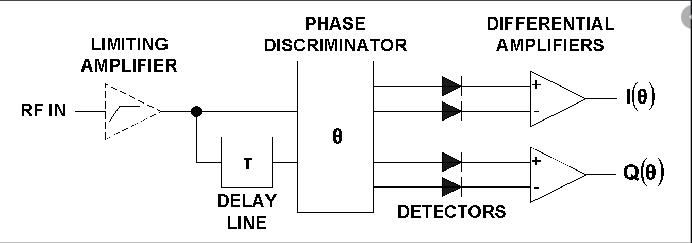
\includegraphics[width=12cm]{Pictures/IFM receiver.png}
    \caption{IFM receiver}
\end{figure}
\newpage
\section{Folding receiver}
In EW scenario is required a solution with high sensibility and which gives the possibility to search in the whole bandwidth at the same time, the folding channeled receiver is suitable for this case. It's important to note that whit the precedent implementations (super het and IFM receivers) is possible to perform a scan of a bandwidth's portion per time in order to achieve a scansion of the whole bandwidth but in different moments. So by using for example the super het receiver the requirements of high sensibility and possibility to make measurements are met. To met also the requirement to have at the same time the possibility to look in the whole bandwidth simultaneously, so to have a POI parameter about one, is possible to put in parallel such devices and that is exactly what the folded receiver does. Such device is implemented by a N-plexer with a bench of low pass filter each tuned with a fraction of the whole band in order to achieve a reconstruction of it by summing their N result. In this way the noise significantly increases (N time) so it is possible to avoid this worsening effect by putting N amplifier after the bench. If these are put before, the problem of high power signals (saturation) and unwanted intermodulation shows up again (wide open limitations). After the bench and the amplifiers there is a problem of receiver structures that follow. Is extremely costly to have N parallel receiver structure, so to avoid this possibility each amplifier is followed by an IF translator (mux plus LO) and the result of each component is summed up, obtaining in this way the whole IF bandwidth. Here there is the 'folding' suggested by the name of this receiver, each fraction of the total band (coverage band) is converted in IF domain and then folded in a single band. 

\begin{figure}[h!]
    \centering
    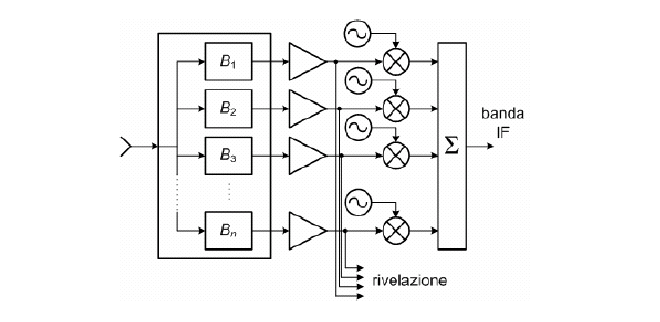
\includegraphics[width=12cm]{Pictures/channeled receiver.png}
    \caption{Folding receiver}
\end{figure}

After this receiver stage come into play other devices to better perform measurements to each signal, compare result with stored information to understand the possible threat. All these actions are better performed in a digital domain. This digital conversion years by years is getting closer to the antenna thanks to the Digital Signal Processors (DSPs) and the Field Programmable Gate Arrays (FPGAs).
\newpage
\section{Shared apertures} The last evolution of receiver-transmitter front end is performed by the phased array antennas. Thanks to this solution is possible to implement a directional single or multi beam in order to obtain with the same device both ECM and ESM action in a time sharing way. The difficult in this case is presented by the fact that the two action requires contrasting features like spectral purity, low noise and lateral lobes for radar (ESM) and large bandwidth and flexibility for defense (ECM). The possibility to commute the beam in microseconds is the feature that permit to share the same hardware in time division for different purpose. The initial difficulties in the development of this technique were strictly technical. The tools had to be very large and bulky. Then the development of digital technology has effectively eliminated this problem thanks to the possibility of having a very high digital resolution without increasing the noise too much. Then the second difficulty was to create a single system with ECM and ESM features based on the same hardware and use it in different time instants, in this regard, shared apertures are used to carry out tracking, surveillance and disturbance actions in deferred time. Now it is possible to focus on the specific characteristics of the different ESM and ECM actions that the hardware must satisfy at the same time. \newline As for the bandwidth, a typical radar system needs about 10 or 15\% of the center frequency (All the frequencies for which the gain is in range max +-3dB, for example 1 GHz in X band) while a typical ECM system works on a much wider band (2-18 GHz). In this case, it is usually decided to use a wideband solution such as to satisfy the ECM requirements and also bring benefits to the radar application as regards the multipath propagation. For example, by doubling the frequencies, the points of constructive and destructive interference are inverted, thus making them more easily identifiable.\newline As regards the spectral purity, it is necessary to keep the transmitted signals under control for the two different applications (ECM and ESM). For a radar, transmitting a noise means finding it in the return echo without having the possibility of being able to filter it (clutter removal and doppler filtering). While transmitting noise is the main ECM technique used. \newline The lateral lobes level in ECM is important for efficiency, to avoid reflection and so interference on the main lobe. In radar and so in ESM lateral lobes are important for anti clutter technique but are less important if we consider that one of the most used jamming technique interest the lateral lobes (Angle deception jamming). So the decision of design it must be taken considering the context and the main objective of the device. Concept that extends to the entire design of shared apertures, it is necessary to consider the context and the main objectives to design the characteristics such as bandwidth, spectral purity and lateral lobes. It is certainly possible to implement a work on differentiated bands for the various functions (ECM, ESM and ECCM)

\begin{figure}[h!]
    \centering
    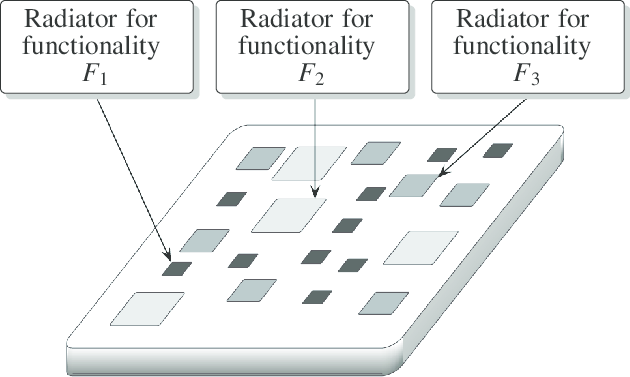
\includegraphics[width=12cm]{Pictures/Illustrative-for-the-shared-aperture-antenna-concept-different-sets-of-radiators.png}
    \caption{Shared apertures example}
\end{figure}



Articles \cite{ewsys} \cite{radarsys} \cite{wiki:ew}

\chapter{ECM and ECCM} \label{Electronic Attack}
Coming now into the details of Electronic Attack (EA) subdivision is possible to better describe and understand how the the different system work.
\section{On board and off board ECM}
 For what concern the ARM category mentioned in the first chapter, this technology is well confirmed and also if it is costly, is also particularly effective. Practically the missiles are equipped by a seeker tuned on the radar emitter enemy that guide the weapon where the gain of receiver signal increase. The winning approach of this solution is  given by the fact that the radar cross section of such weapon is very low and consequently is very difficult to contrast it. But not only the dimension are influential in this case also the front end of the missile, that is matched with the enemy emitter, reflect only the dismatched energy. \newline For what concern the passive on board techniques the most used is the signature reduction. The goal of this practice is to reduce the radar cross section of the system equipped. The reduction is achieved by an appropriate profile design and by using absorbent materials. Is important to note that this stealth technology is effective only against monostatic radar configuration and in small range bandwidth, because is difficult to use materials that absorb energy coming from a large set of frequencies. \newline For the passive off board systems in precedent chapter mentioned, chaff and decoy, are better described now. Chaff technique is the emission of metallic stripes with high reflectivity in order to generate a clutter that disturb enemy radar. Decoy are single reflective elements like corner reflector, in order to seem real targets through which it is possible to divert the enemy's attention. \newline The active off board systems are instead separated emitters that produce electromagnetic signals in order to disturb enemy radar  with a jamming approach. The most simple active off board system is just a repeater, moreover there are expendable and towed system. The first are in free evolution in the space while the towed are controlled. \newline For the active on board techniques the most used systems are based on the jamming approach. In particular is possible to distinguish three different kind of jamming approach:
\begin{itemize}
     \item Self screening jammer: 
         \begin{itemize}
         \item In which the system equipped with use his own ECM instruments to generate disturbing signals. Cons of this implementation is the costly in terms of weight and volume that increase significantly. For what concern the pros, there is secure effectiveness of jamming and the minimal request of energy.
         \end{itemize}
    \item Escort jammer: 
         \begin{itemize}
         \item In this case the ECM instruments used to perform the jamming technique are on a second platform that follow the principal one and escort it. The benefit is that the principal platform or system is light and less expensive in terms of instrumentation. But on the other hand there are two platforms exposed to enemy.
        \end{itemize}
    \item Stand off jammer:
         \begin{itemize}
         \item Dedicated platform with ECM instruments is used to perform the jamming technique, but in this case it remains in a fixed position far from enemy area. In this case high energy is required to reach the zone of action and always more than one platform is necessary to cover a reasonable area.
         \end{itemize}
\end{itemize}
Not only jamming but also meaconing and spoofing approaches are used for what concern active ECM systems and in particular these are very suitable in the case of GNSS signals. Meaconing is the action of interception and rebroadcast of GNSS signals with more power in order to confuse enemy navigation. Spoofing is the technique through which fake GNSS signals are forged or original signals are intercepted and modified in order to confuse enemy navigation systems.
 \section{Active ECM}
 When thinking about jamming techniques it is natural to think that the disturbance produced by the ECM system is carried out on the main lobe of the victim signal (enemy radar). This type of attack is produced keeping aligned the two main lobe of enemy radar and ECM system. Considering that not only the main lobes are use by a radar, one of the most effective ECMs against detection radars is the 'sidelobe disturbance'. In such a way as to generate an angular disturbance and make the victim believe that the target is in an incorrect angular position. \newline Another active disturbance approach is offered by the so-called 'repeater jammer', essentially consists in intercepting the victim signal and repeating it in an elaborate way and with more power. If we think to the telecommunications systems this type of attack follow the same concept of the 'replay' attack. The device used for the implementation of this type of attack is Digital Radio Frequency Memory (DRFM) which stores the signal in digital form and then reproduces it in a coherent way. The best known active ECM technique is, as previously mentioned, the noise jammer. By transmitting a thermal noise like signal, the ability of the victim device to detect targets with good sensitivity is inhibited. This is possible because the false thermal noise transmitted is substituted in the calculation of the signal to noise ratio by the victim. There are 2 possible implementations of ECM noise jammer: the 'Spot noise' configuration and the 'barrage noise' one. In the first, the system transmits noise in a narrow band, thus concentrating the energy in a relatively small portion of the band. In the second case, the noise energy is distributed over the entire working band of the victim device. A further possible specific mode of operation of barrage noise conf. is the 'swept noise' in which a frequency modulated CW signals are used in order to generate  continuously a disturbance in each repetition time. The following figure shows a typical example of a spectrum in a situation of spot jamming and barrage jamming. Depending on the situations and the contexts, it is more effective to use one of the different techniques. This mainly depends on the type of device to be countered. 
 
 \begin{figure}[h!]
    \centering
    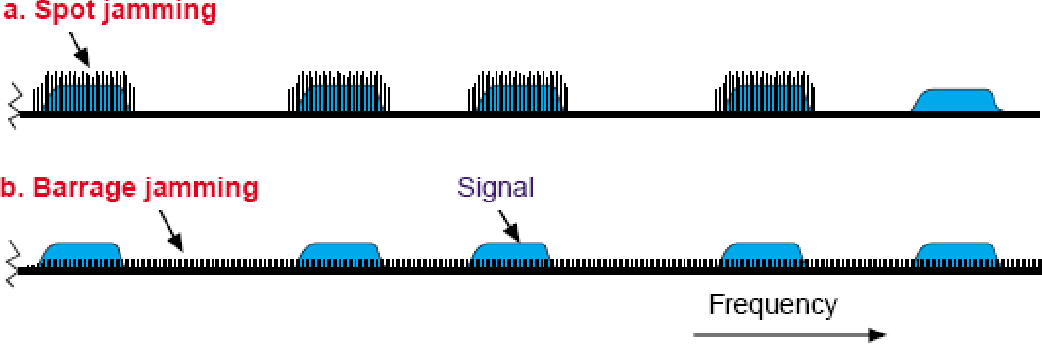
\includegraphics[width=12cm]{Pictures/spot_and_barriage_jamming.png}
    \caption{Spot and Barrage Jamming}
\end{figure}
 
One of the main threats in electronic warfare is represented by automatic pursuit weapons, as in the previously analyzed case of self-guided missiles. Other important active ECM techniques are mentioned against this type of threats. The main objective is to 'unhook' the pursuit of the enemy in distance (range) and speed. In this regard, the 'Range Gate Pull Off' and 'Velocity Gate Pull Off' techniques are used. In the first case, a progressive delay instant after instant is superimposed on the echo produced towards the victim system which, once eliminated, causes enemy release. In the second case is performed the same procedure but this time in the speed tracking loop of the enemy system. (in the previous case the delayed signal is inserted into the distance tracking loop, so in the amplitude measurements of the enemy). In this case using a signal with a frequency close to the real one but which changes progressively. (Considering that the speed in the radar field is obtained by the frequency of the signals, so now the target are the frequency measurements of the enemy).
\newpage


\section{ECM against GNSS/GBAS}
The Global Navigation Surveillance System (GNSS) is vulnerable to various types of electronic attacks, in this case specific to the particular application. This demonstrates how the field of ECMs is variable and depends mainly on the particular system one intends to attack. In this case the attacks are subdivided, as previously mentioned, in three category: jamming, spoofing and meaconing.  In general the EAs used can be expensive in the case of military level or very cheap and widely available like personal protection devices. The most critical attacks have been observed at the level of Ground Base Agumentation Systems, in case they are used as a landing system in conditions of poor visibility. The structure of the GNSS signals and their subdivision in frequency (L1,L2,L5,E1/E2) is well known, but above all the low power with which these are received makes the GNSS vulnerable to the previously mentioned ECMs. Much more resistant to jamming and derived type of attacks are the P/Y code used in GPS (military code). To cover such a long distance it is mandatory to use receivers capable of picking up a low signal power, and it is also one of the main reasons why a code division multiple access technique is often used. In the case of GBASs, the potential vulnerability exposes a much more critical problem than other applications when they are used for Safety of Life services such as emergency landings in critical conditions. In these cases, another point against the GNSS/GBAS is that these stations occupy a fixed and well known position on the ground. In the study of possible attacks on GNSS/GBAS systems it is appropriate to observe some similarities, the first concerns jammming attacks which are similar to a destructive interference between two signals out of phase by 180 degrees and the second concerns spoofing and meaconing which appear to be similar delaying the original signal in order to alter the position and time estimates. Three different methods of protection against these types of attacks are proposed below, the receiver-based mitigation methods, antenna-based methods and the siting-based methods. 

\subsection{GNSS real cases of failure}
It is important to know that even in the case of unintentional disturbances, the surrounding radio scenario is full of devices transmitting and receiving simultaneously that can lead to a degradation of the GNSS signals such in accuracy which leads to a complete failure of the GNSS systems. The key issue, however, as widely seen so far in electronic warfare, is the intentional disturbance of signals using very expensive devices that are part of the war crews or very low cost and widely available devices. The first major example of complete failure of the navigation systems occurred on November 8, 2018 during a NATO exercise in Finland that resulted in the collision between a frigate and a tanker. Other systems operating in the vicinity of the incident have confirmed problems in GNSS applications. Other experiences, even more confirmed and ascertained due to disturbing actions against the GPS signal, occurred in South Korea and Ukraine between 2010 and 2013. In this case, the disruptive actions were deliberately produced by North Korean military jammers against aircraft and ships. While in Ukraine the jamming actions are reported against UAVs (Unmanned Aerial Veichles). The effect to keep more under control is the jamming produced by low cost devices called Personal Protection Devices (PPD), easily available in the internet market. Anyone with these devices could be able to produce distorting effects against GNSS applications. This type of disturbance is experienced and confirmed at Newark Liberty International Airport/USA in 2012. In this case the source of disturbance was found to be a truck jammer driving nearby the airport. Therefore observing from the specific point of view for the GNSS/GBAS the electronic attacks ECM/EAs and the electronic defense ECCM are intended as the interruption of the relative signals or their protection. In particular the EA is performed by degrading, disrupting, or deceptively manipulating positioning, navigation and timing transmissions.
\subsection{GNSS/GBAS signals and architecture}
Specifically analyzing the GBAS system (Ground Based Agumentation System), a system of base stations on the ground used to increase the accuracy of the information coming from the GNSS signal by reducing the error. Thanks to the fixed and known position, the signal received in fixed stations can be compared with the signal received from nearby mobiles, in order to better estimate the error and eliminate it from the end user's signal. Furthermore, this station system that allows to achieve high performance in terms of accuracy can also be used as a support tool for critical and more important operations such as an emergency landing. In this scenario, four different radio links between the various systems can be classified. These systems are the satellites, the aircraft, the GBAS station and the ATC (Air Traffic Crontol) and four radio links between these are the follow:
\begin{itemize}
     \item Satellite - GBAS ground station link, it is a vulnerable link due to the low power of the received signal (about -160 dB) with a consequent very low Signal to Noise Ratio. In this case, protection techniques are used such as low probability of intercept (LPI) signals by energy spreding along the entire spectrum.
         
     \item Satellite - Aircraft link, it is a stronger link against electronic attacks thanks to the altitude of the aircraft and its moving position at high speed. To disturb this link very expensive tools such as UAV jammers or other aircraft used to disturb communication are required.
         
     \item GBAS ground station - Aircraft link, it is a stronger link against electronic attacks thanks to strong energy transmitted that permits to achieve an high signal to noise ratio.
        
    
     \item GBAS station - ATC link, that is a fixed link to only control and manage the status of the entire system.
        
\end{itemize}
In the follow picture are presented an usual case of implementation in airport of GBAS system.
 \begin{figure}[h!]
    \centering
    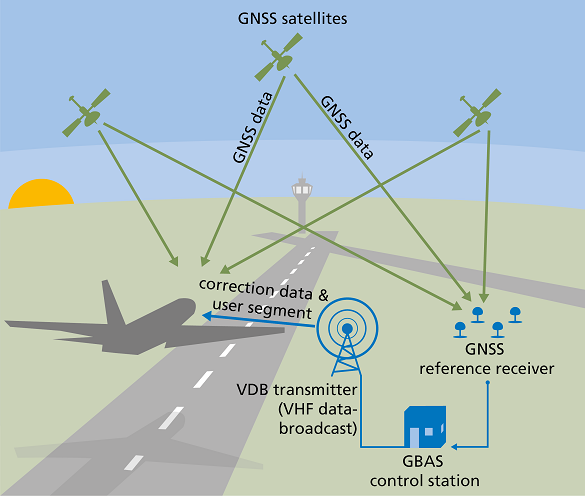
\includegraphics[width=9cm]{Pictures/GBAS_GNSS.png}
    \caption{GNSS/GBAS Arch.}
\end{figure}

Analyzing the signal produced by the satellites and therefore coming from the space segment, in the GPS case there are two different carrier frequencies and two different codes used. (Remembering that the type of multiple access transmission is based on the use of PRN sequences, to ensure almost no interference between the multiple signals by spreading the energy - spread spectrum communications system). Each PRN code is unique for each satellite. The first type of codes used is the C/A coarse acquisition code repeated every millisecond and known to all, used for civil purposes. The second type of codes is the P code, repeated over a much larger time interval (approximately 266 days) providing greater accuracy along with safety. It is also used for military purposes in its anti spoofing version in which the P code is the result of the Y code encrypting through exclusive sum with the W code (secret encryption code). PRN codes are generated by tapped feedback shift registers. Navigation messages from satellites contain various information such as satellite status information, clock information, orbit information, correction data. Ephemeris data are very important information on the position of satellites, mainly used by receivers to calculate the position. This data mainly concerns GPS, the US GNSS tool, while the counterparts Galileo (EU), GLONASS (RU) and Beidou (CN) use the same principles for calculating the position with different signal structures.
In the next picture are listed the different bands used by the different GNSS system. 

 \begin{figure}[h!]
    \centering
    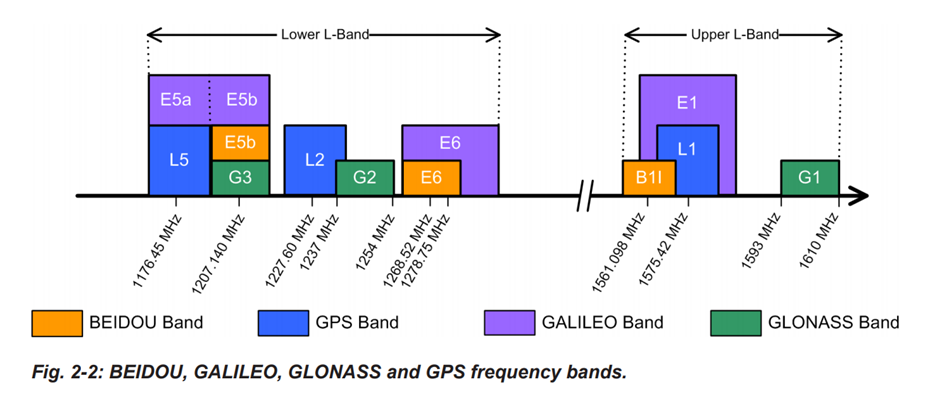
\includegraphics[width=16cm]{Pictures/frequencies.png}
    \caption{GNSS freq. subdivision}
\end{figure}

The following image shows the power spectrum density of the signals used by the different GNSS systems.

 \begin{figure}[h!]
    \centering
    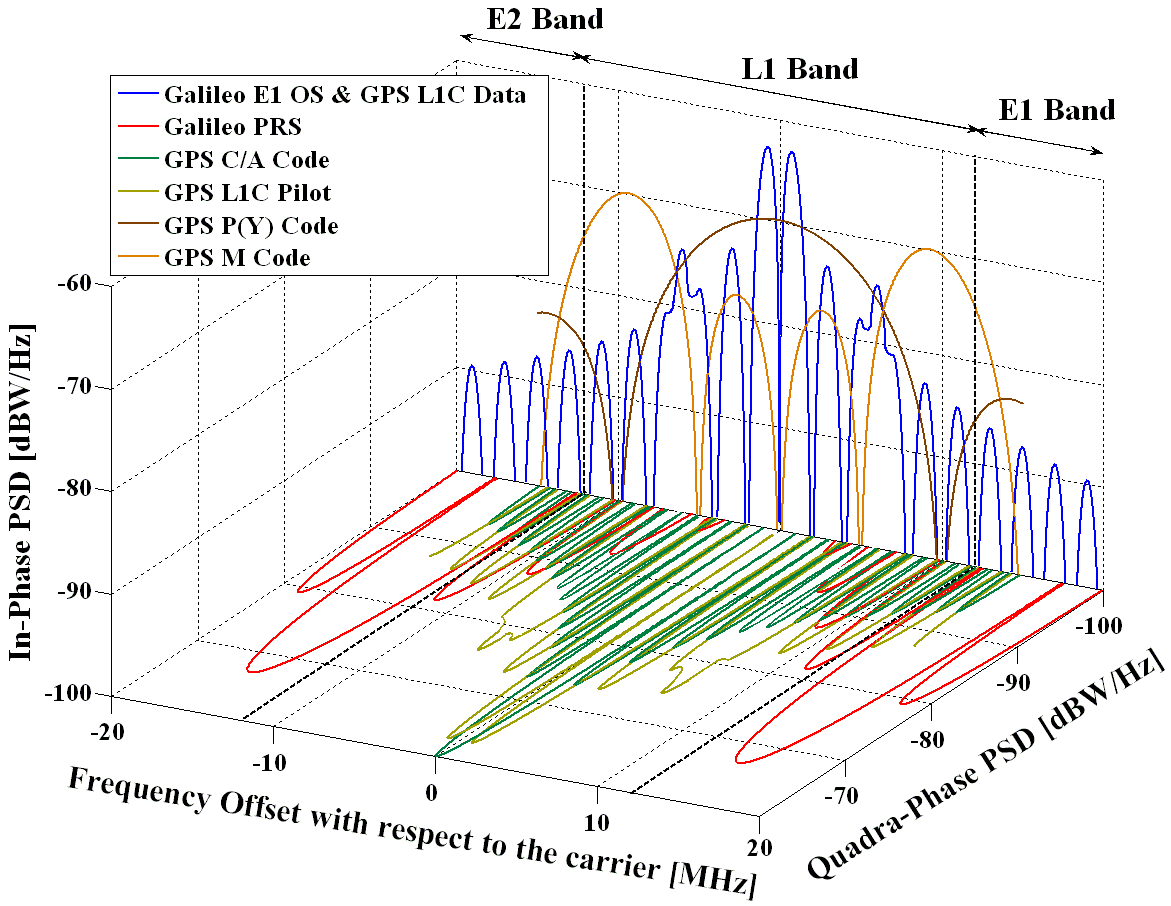
\includegraphics[width=16cm]{Pictures/Galileo_Signal_Plan_Fig_3.png}
    \caption{GNSS I,Q PSD}
\end{figure}

All the satellites of a constellation transmit the signals at the same frequency and thanks to the spreading codes the receivers can select the satellites in sight and not only, the direct spread spectrum technique allows to have a starting base of LPI (Low Probability of Intercept).
In the following subchapter a possible jamming model is considered and described, that is the first type of possible electronic attack against the GNSS mentioned above. The subsequent types of attacks such as spoofing and meconing can be considered simpler from the implementation point of view in the case of unauthenticated and non-integrity messages. In particular, meaconing is considered the younger brother of spoofing as it involves resending the messages already produced by satellites (dual concept of the replay attack in a telecommunications network). Both types of spoofing and meaconing can be successfully mitigated by implementing an authentication and message integrity system. In particular, by adding a fresh, new and completely random value to each message and by calculating a hash, it is possible to verify that each message has not been tampered with or resent for a second time.

\subsection{Jamming model}
To better describe the effects of jamming, a mathematical model can be used which has as its main parameter the expression of the jamming to useful signal ratio, shown below: $J/S = ERP_{j} - ERP_{s} - L_{j} - L_{s} + G_{rj} - G_{s}$ 

\begin{itemize}
     \item $J/S$: The ratio between jamming signal power and useful signal power expressed in dB;
         
    \item $ERP_{j}$: The Effective Radiated Power of jamming signal expressed in dBm;
        
    \item $ERP_{j}$: The Effective Radiated Power of useful signal expressd in dBm;
         
    \item $L_{j}$: The propagation loss derived from the path between target and soruce of jamm expressed in dB;
        
    \item $G_{rj}$: The receiving antenna gain of the jammer antenna expressed in dB;
           
    item $G_{s}$:  The receiving antenna gain of the useful target signal expressed in dB;
               
\end{itemize}
The greater the ratio between the jamming power and the victim signal, the better the destructive effect will be. Observing now, as previously introduced, the effect of jamming as interference coming from multipath, it is possible to identify spoofing and meaconing as constructive interference and actual jamming as destructive interference. Recalling the fundamental principles of physics, constructive interference occurs when the two signals that meet at a point in space have the same phase (zero phase difference) while destructive interference occurs when they are in phase opposition (difference phase equal to 180 degrees). Specifically analyzing a typical GNSS signal where $d(t)$ indicates the signal containing the data, with $c(t)$ the signal containing the code used, and the in-phase carrier as an example which depends on the type of modulation used. The following signal occurs: \newline \newline
$r(t) = A_{0} d(t - \tau_{0}) c(t - \tau_{0}) \cos({2\pi f_{L1}t - \theta_{0}}) + A_{1} d(t - \tau_{1}) c(t - \tau_{1}) \cos({2\pi f_{L1}t - \theta_{1}})$ \newline \newline
The therms of amplitude, phase and delay of first member in the equation belongs to the useful signal while the second therm member represent the designed jamming signal like the multipath reflected signal. By accurately chooses the values of amplitude, delay and phase constructive or destructive interference is achieved. By using an appropriate multipath model, exponential model, and by running some experiments by reproducing the GNSS signal superimposed with the multipath signal the followed result are achieved by the analyzed paper \cite{gnssgbasattack}.
Is important to consider always the constructive and destructive interference as the EAs considered spoofing, meaconing and jamming achieved simple by suitable choice of the amplitude, phase and delay terms of the second member in the last equation in multipath condition.

\begin{figure}[h!]
    \centering
    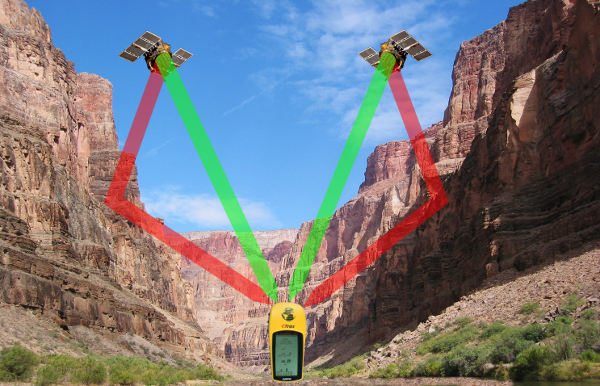
\includegraphics[width=10cm]{Pictures/Gps-multipath-efect.png}
    \caption{GPS multipath effect}
\end{figure}

The results obtained from the analyzed paper show that the Galileo constellation manages to maintain very good results even in multipath conditions both in Europe and in the USA with $99.99\%$ and $99.75\%$ probability of accuracy respected in cat. 3. While the GPS does not appear to have sufficiently stable areas in which similar results can be obtained. 
\subsection{Mitigation methods}
Three different types of mitigation mechanisms can be used to cancel the effects due to the EAs in question:

\begin{itemize}
     \item Receiver based technique;
         
    \item Antenna based technique;
        
    \item Sitting based technique;
\end{itemize}

The first group of mitigation techniques is based on the implementation of further processing carried out on the signal in the receiver. In addition to the standard correlator which measures the autocorrelation every chip time (1 chip) with the early-gate window, a Narrow Correlator is inserted in which the chip spacing is 10 times smaller (0.1 chip). Another feature that can be monitored is the signal structure using BOC (Binary Off Set) modulations that place some additional power at the high frequencies to allow for better tracking once the signal is acquired. The second type of methods directly concerning the construction of the receiving antenna provides for the creation of nulls in reception towards the probable jamming/multipath directions. (Thus creating antennas capable of receiving only from a certain direction rather than from all directions). These type of antenna are Flat Antenna Array, Curved Antenna Array Stack Antenna, and the Array Curved Antenna Array. The last method is the sitting criteria, concern the position of GBAS station in order to avoid reflection and interference by another transmission and so the multipath negative effect. \newpage
\section{Electro Magnetic Pulse}
As seen so far, all of the tools and devices used in the field of electronic warfare fully rely on electronic management. Even the most sophisticated devices use microprocessor and micro controller technology. Therefore dealing with the topic of ECMs and ECCMs it is appropriate to consider the electromagnetic pulses used as a means of electronic attack. \cite{emp2} The main effect obtained through the use of this practice is the born out of all electronic devices present in a certain range of action. The forced choice for each device falls on the use of micro electronics including the most modern and avant-garde devices. This makes electromagnetic pulses one of the most destructive and terrifying electronic weapons compared to all the others thanks to the ability to inhibit any enemy function in any area. In particular, electromagnetic pulses fall within the set of direct energy weapons in the context of electronic warfare. While on the one hand the research is aimed at the offensive capacity of the electromagnetic pulse (ECM), on the other hand it is strongly aimed at finding a defensive solution against this type of attack (ECCM). The use of ferromagnetic cages as defensive shields against electromagnetic pulses is known, but although it is particularly effective for this purpose, it is difficult to install and it is practically impossible to equip to each electronic device. More specifically, the electromagnetic pulse is a burst of electromagnetic radiation. In fact, the first experiments made by USA starting from the Second World War led to the creation of an EMP (Electro Magnetic Pulse) starting from a nuclear explosion. In particular, an EMP is obtained by generating a nuclear explosion at high altitude, hundreds of km of altitude. The very strong and rapid variations of the electric and magnetic fields that follow cause destructive currents and voltages in the electronic devices. The most resonant of the experiments conducted by the united states in 1961 is called the Starfish Prime Test in which a 1.44 megaton hydrogen bomb was used. The destructive effects derived from the consecutive EMP were felt up to 1845 km away, about 898 nautical miles. The main effects were those of burn out of all street lights, complete blocking of a telephone company and various alarms in the area. The similar experiments that followed were particularly important because they allowed the researchers to fully understand the phenomenon and allowed to recreate the situation without the need for an explosion. The important result is to be able to create EMPs simply by means of devices and electricity. The first laboratory in which an artificial EMP (without the aid of an atomic explosion) was the 'White Sands Missile Range' in America. The device capable of recreating the EMP is a giant cylinder containing the windings of a reel capable of creating the impulse with pre-established parameters on a certain area, called EMP discharge device. In the experimentation area are placed the electronic tools that you want to protect such as military vehicles, airplanes and computers in order to study their effects and understand the necessary ECCM. The next figure shows the device in question during a test performed on an airplane. 

\begin{figure}[h!]
    \centering
    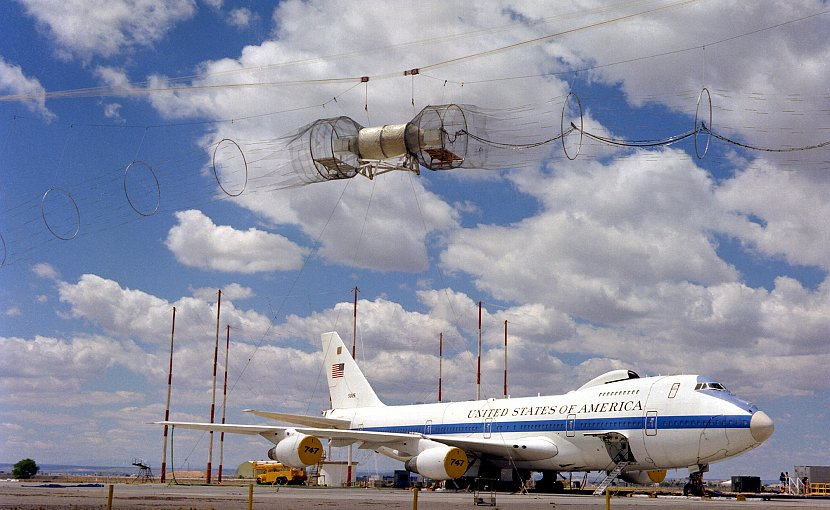
\includegraphics[width=10cm]{Pictures/EMP test.jpg}
    \caption{EMP test on aircraft}
\end{figure}

As for the experimentation and creation of an EMP in general, they can be created by 3 different phenomena:

\begin{itemize}
     \item Geomagnetic solar storms;
         
    \item Nuclear explosions;
        
    \item EMP discharge devices;
\end{itemize}

The effects derived in an EW context are the most feared, first of all the complete cancellation of the enemy electronic functions or the functionality of almost all devices. Regarding the experiments conducted in the paper studied \cite{emp1}, the EMP discharge devices can be obtained according to two different electronic types: the battery Tesla coil and the battery Marx generator. The Tesla coil consists of a primary transformer, a high voltage capacitor, a spark gap, and a toroid design. During the initial phase the voltage is gradually increased between the two ends of the spark gap through the high voltage transformer until they begin to ionize the air. Then the spark gap tends to act as a switch to let the current flow and the capacitor discharges, generating the EMP. In the paper's experiment an AA battery is used and a coverage area of 1 m of diameter is achieved. While as far as the battery Marx generator is concerned, the Marx generator is a device used since 1924 to generate high voltage pulses useful for testing the resistance of power lines and aircraft to lightning. As previously anticipated, an excellent method to protect devices from this type of attacks is the use of a magnetic iron cage, such as the Faraday cage. The relevant feature of this type of protective shield lies in the fact that it does not block static or quasi-static fields such as the terrestrial one, consequently a compass inside it continues to work safely and at the same time is protected by EMPs. But its protective operation is not always guaranteed, it depends primarily on the thickness of the cage and its measures. In particular, if the distance between the openings is not significantly smaller than the wavelength of the EMPs radiation, it does not protect the devices at all. A typical example of this solution is shown in the protection of forensic computers that require a space free from all electromagnetic radiations, for this reason they are installed in rooms covered with one or more layers of perforated metals capable of shielding any external radiation. At the same time it is possible through this example to understand how difficult it is to implement a solution of this type for all the devices used and employed in electronic warfare. Especially with regard to the design and implementation costs on each device. A simpler solution to implement and to sustain in terms of costs, is a device capable of detecting the presence of an EMP and in general an anomalous external electromagnetic radiation. In this way, if the device in question is able to detect the imminent arrival of an EMP, you have time to switch off or protect the electronic devices. This completely reduces the cost of designing and implementing a Faraday cage for each device and at the same time offers a mobile and flexible solution to this problem.

\section{Conclusion}
What we have seen so far shows how electronic warfare has a relevant importance nowadays. In particular, thanks to continuous technological innovation and the use of increasingly sophisticated instruments that integrate more and more functions in the least possible hardware, an easy transport and ease of installation are made possible. Starting from the receivers, key devices of the subject matter, and ending with direct energy weapons such as the EMP, the knowledge of the architecture of the devices and of the technology used so far is essential to be able to increase the value by favoring research and Development. The concepts and definitions of electronic warfare also affect instruments for civilian use such as GNSS, also used in particular and sensitive situations such as in the GBAS landing case. It is therefore mandatory to consider the possible EW practices when designing emergency and sensitive electronic systems as in the case of safety of life applications. Furthermore, as a last consideration it is of crucial importance to remember that all the operations carried out in daily life now take place in a digital domain, exposing almost all the actions carried out daily, telecommunications, navigation, etc ... to the possible practices of EW, this demonstrates the importance of knowledge in this field.

\listoffigures
\bibliographystyle{unsrt}
\bibliography{biblio}
\end{document}
